\section{Auswertung}

\section{Auswahl der NV-Zentren}
Im Versuch wurden zweimal ein NV-Zentrum und anschlie\ss end die hellste Lichtquelle analysiert.
Die Abbildungen \vref{fig:NV} und \vref{fig:hell} zeigen, wie die Messpunkte in der Probe ausgew"ahlt wurden.
\begin{figure}[htbp]
    \begin{subfigure}[t][][b]{0.43\textwidth}
        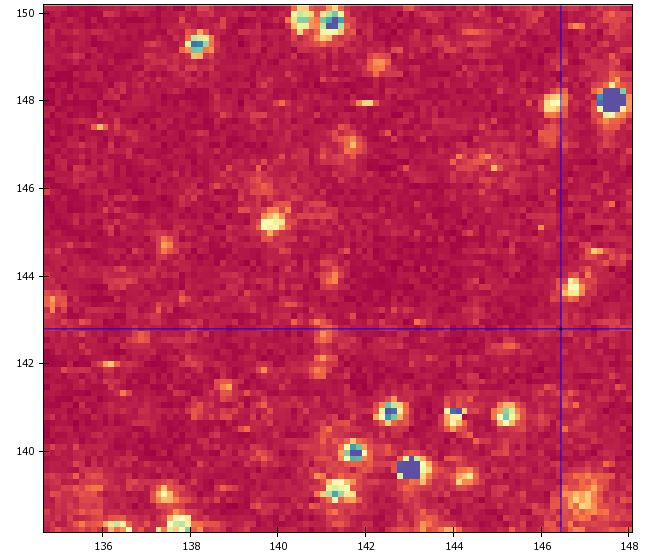
\includegraphics[width=1\textwidth]{messung_1.JPG}
        \subcaption{Messung: NV-Zentrum 1 (NV 1)}
        \label{fig:NV:1}
    \end{subfigure}
    \begin{subfigure}[t][][b]{0.42\textwidth}
        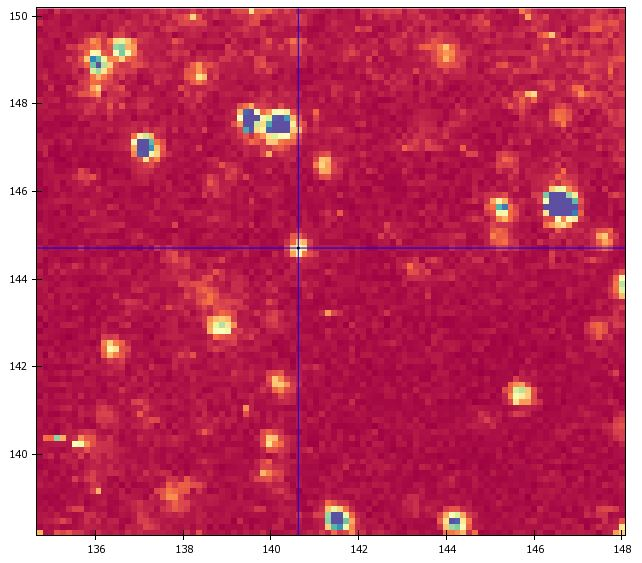
\includegraphics[width=1\textwidth]{messung_2.JPG}
        \subcaption{Messung: NV-Zentrum 2 (NV 2)}
        \label{fig:NV:2}
    \end{subfigure}
    \hfill
    \begin{subfigure}[t][][b]{0.1\textwidth}
        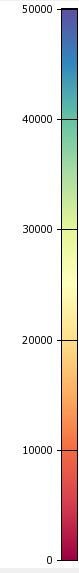
\includegraphics[height=3.6\textwidth]{skala_1_2.JPG}
    \end{subfigure}
    \caption{
        Die Abbildung verdeutlicht, wie die NV-Zentren f"ur die Messung ausgew"ahlt wurden.
        Die Graphiken zeigen dabei die Intensit"atsverteilung der Lichtemission in der Probe.
        Einzelne NV-Zentren sind diejenigen Punkte, die von den anderen separiert sind, keine zu hohe Intensit"at haben und im Zoom etwa kreisf"ormig erscheinen.
        Das blaue Fadenkreuz zeigt jeweils an, welches Zentrum f"ur die beiden Messungen ausgew"ahlt wurde.
        Die Messungen werden NV 1 und NV 2 genannt.
        Bei NV 1 liegt das Fadenkreuz nicht mehr ganz auf dem Punkt (rechts "uber dem Fadenkreuz).
        Dies liegt daran, dass das Bild erst am Ende der Messung aufgenommen wurde.
        Die Intensit"atsverteilung zeigt dabei die Situation zu Beginn und das Fadenkreuz die Position des NV-Zentrums nach etwa zwei Stunden.
        Es ist um einiges gewandert.
        \\
        Zur Skala: Die Angaben an den Bildern sind in \si{\nano\metre} und die Intensit"atsskala ist in \si{counts\per\second} gegeben.
        }
    \label{fig:NV}
\end{figure}
\begin{figure}[htbp]
        \begin{subfigure}[b][][t]{0.43\textwidth}
            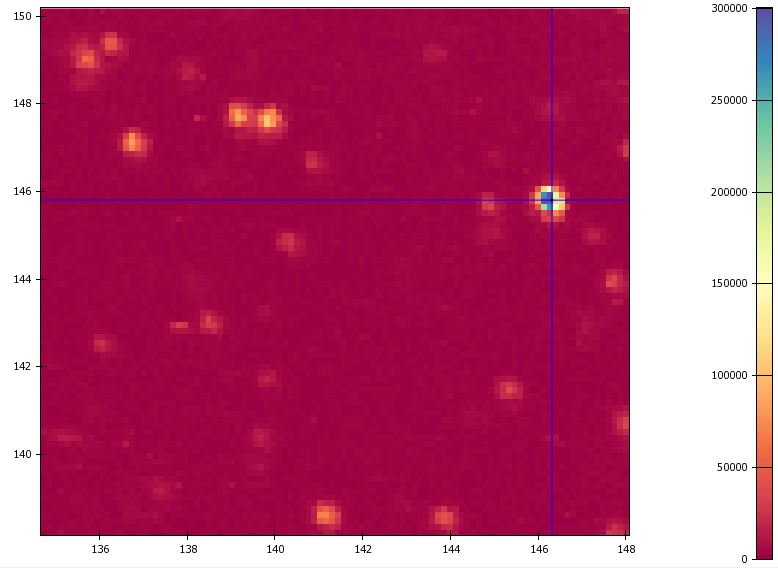
\includegraphics[width=1\textwidth]{messung_3.JPG}
        \end{subfigure}
        \hfill
        \begin{minipage}[b][][t]{0.5\textwidth}
            \caption{
                Messung: Hellster Punkt (HP)
                \\
                Zus"atzlich zu den NV-Zentren wurde noch eine weitere Lichtquelle untersucht.
                die nebenstehende Abbildung zeigt, wie der hellste verf"ugbare Punkt als Quelle ausgew"ahlt wird.
                \\
                Zur Skala: Die Angaben an den Bildern sind in \si{\nano\metre} und die Intensit"atsskala ist in \si{counts\per\second} gegeben.
                }
            \label{fig:hell}
        \end{minipage}
\end{figure}

\subsection{Berechnung der Korrelationsfunktion}
\begin{table}[htbp]
    \caption{
        Die Tabelle zeigt die Z"ahlraten $N_1$ und $N_2$ der Detektoren die zu einem Zeitpunkt w"ahrend der Messung aufgenommen wurden.
        Ihr Verh"altnis $f=N_2/N_1$ wird direkt daraus berechnet.
        Wie unschwer zu erkennen ist, arbeitet Detektor 2 effizienter als Detektor 1.
        $T$ bezeichnet die Gesamtdauer der Messung.
        }
    \label{tab:counts}
    \begin{tabular}{l|S[table-format=6]S[table-format=6]S[table-format=1.2]S[table-format=4.2]}
        Versuch
            &{$N_1$ [\si{counts\per\second}]}
            &{$N_2$ [\si{counts\per\second}]}
            &{$f=N_2/N_1$}
            &{$T$ [\si{\second}]}\\\hline
        NV-Zentrum 1
            &11000
            &20000
            &1.82
            &6128.2\\
        NV-Zentrum 2
            &12000
            &21000
            &1.75
            &6525.34\\
        Hellster Punkt
            &120000
            &200000
            &1.67
            &460.99
    \end{tabular}
\end{table}
Im Versuch wird ein Histogramm aufgenommen, welches die H"aufigkeit z"ahlt, mit der zwischen dem Klick an Detektor 1 und dem an  Detektor 2 die Zeit $\tau$ vergeht.
Diese Verteilung wird im folgenden $c(\tau)$ genannt.
Zus"atzlich werden die Z"ahlraten $N_1$ und $N_2$ der Detektoren 1 und 2 aufgenommen.
Die aufgenommenen Z"ahlraten sind in Tabelle \vref{tab:counts} eingetragen.
Es zeigt sich, dass diese im Versuch stark variieren; beim ersten Durchgang schwankte $N_2$ zwischen \SI{10000}{} und \SI{30000}{}.
Diese Schwankung ist darauf zur"uckzuf"uhren, dass die NV-Zentren in der Probe wandern und sich so aus dem Fokus bewegen.
Dieser wird zwar alle 3 Minuten neu justiert, aber der Intensit"atsverlust ist dennoch bedeutend.
Um diese Schwankung auszugleichen, wird das Verh"altnis $f=N_2/N_1$ konstant gehalten um die Z"ahlraten anschlie\ss end so zu optimieren, dass die Korrelationsfunktion $g^{(2)}(\tau)$ f"ur gro\ss e Zeitdifferenzen $\tau$ zu $g^{(2)}(\abs{\tau}\gg \tau_\text{c})=1$ wird, wobei $\tau_\text{c}$ die Korrelationszeit ist.

Die Korrelationsfunktion wird folgenderma\ss en berechnet.
Zuerst wird die Verteilung $c(\tau)$ normalisiert.
Dies geschieht "uber
\begin{equation}
C_\text{N}(\tau)
    =\frac{c(\tau)}{N_1N_2\omega T},
    \label{eq:CN}
\end{equation}
wobei $\omega=\SI{0.5}{\nano\second}$ die Breite der Zeitintervalle f"ur die Verteilung und $T$ die Gesamtdauer der Messung ist (siehe Tabelle \vref{tab:counts}).
Anschlie\ss end wird die Hintergrundstrahlung abgezogen.
Die Intensit"at $B$ der Hintergrundstrahlung wird durch Messung an einem Punkt in der Probe mit m"oglichst niedriger Intensit"at bestimmt zu $B=N_1^{(\text{B})}+N_2^{(\text{B})}=\SI{1100}{counts\per\second}$, wobei $N_i^{(\text{B})}$ die Z"ahlraten der Detektoren sind.
Die Signalst"arke einer Messreihe berechnet sich zu $S=N_1+N_2-B$.
%\begin{align}
%S
%    &=N_1+N_2-B;
%    \label{eq:S}\\
%S^\text{(NV 1)}
%    &=\SI{11000}{counts\per\second}+\SI{20000}{counts\per\second}-\SI{1100}{counts\per\second}
%    \nonumber\\
%     &=\SI{29900}{counts\per\second}.
%     \nonumber
%\end{align}
Die Korrelationsfunktion wird dann
\begin{equation}
g^{(2)}(\tau)
    =\left[ C_\text{N}(\tau)-(1-\rho^2)\right]/\rho^2,
    \label{eq:g2}
\end{equation}
mit $\rho=S/(S+B)$.

F"ur eine Poissonverteilung der Strahlungsquelle wird eine Korrelationsfunktion der Form
\begin{equation}
g^{(2)}(\tau)
    =h-(h-a)\cdot \exp(-\frac{\abs{\tau}}{\tau_\text{c}})
    \label{eq:fit}
\end{equation}
erwartet, wobei $a$ die Korrelation bei $\tau=\SI{0}{\second}$, $\tau_\text{c}$ die Korrelationszeit und $h$ der Wert der Funktion im unendlichen ist.
Diese Gleichung wird an die Daten \eqref{eq:g2} gefittet.

Da die Ereignisse f"ur gro\ss e Zeiten nicht mehr korreliert sind, sollte $h=1$ sein.
Dies ist mit den aktuellen Z"ahlraten ($N_1$ und $N_2$) nicht der Fall.
Aber aus dem sich ergebendem $h$ k"onnen neue mittlere Z"ahlraten so bestimmt werden, dass das neue $h=1$ wird.
Da die Gleichung nicht trivial nach $N_2=f\cdot N_1$ umgestellt werden kann, werden $N_1$ und $N_2$ zun"achst mit $\sqrt{h}$ multipliziert (das entspricht $C_\text{N}/h$).
Anschlie\ss end werden alle Rechenschritte wiederholt und ein neuer Fit durchgef"uhrt.
Dies wird wiederholt bis $h=1 $ ist.

\subsection{Ergebnisse}
Tabelle \vref{tab:final} zeigt die endg"ultigen Fitparameter.
Dort ist zu erkennen, dass die Korrelationszeiten von NV 1 und NV 2 um das f"unffache abweichen.
Die Abbildungen zeigen, dass die Korrelation f"ur $\tau=0$ nicht ganz auf 0 herunter geht, ja gerade mal auf $0.75$.
Dies konnte durch den m"oglichen Einfluss eines zweiten NV-Zentrums erkl"art werden oder durch eine st"arkere Hintergrundstrahlung als angenommen.

Au\ss erdem sind bei $\tau=\SI{13.5}{ns}$ Peaks in allen drei Korrelationsfunktionen zu erkennen.
Diese sind vermutlich auf die Tatsache zur"uckzuf"uhren, dass ein Detektor wesentlich sensibler ist als der andere.

\begin{table}[htbp]
    \caption{
        Die Tabelle listet die finalen Fitparameter.
        Dabei entspricht $\tau_\text{c}$ der Korrelationszeit, $a$ der Korrelation bei $\tau =0$ und $h$ der Korrelation f"ur $\tau \gg \tau_\text{c}$.
        Die Unsicherheiten entsprechen Standardabweichung beim Fit.
        Au\ss erdem sind die korrigierten mittleren Z"ahlraten $N_i$ aufgef"uhrt.
        \\
        Es ist dabei zu erkennen, dass die Korrelazionszeit f"ur NV 1 fast f"unfmal so gro\ss\ ist, wie die f"ur NV 2.
        Daf"ur ist sie bei NV 2 ungef"ahr so gro\ss\ wie bei HP.
    }
    \label{tab:final}
    \begin{tabular}{
            l|
            S[table-format=6]
            S[table-format=6]
            S[
                table-format=2.1,
                separate-uncertainty,
                table-figures-uncertainty = 1
                ]
            S[
                table-format=1.3,
                separate-uncertainty,
                table-figures-uncertainty = 1
                ]
            S[
                table-format=1.3,
                separate-uncertainty,
                table-figures-uncertainty = 1
                ]
            }
        Versuch
            &{$N_1$ [\si{counts\per\second}]}
            &{$N_2$ [\si{counts\per\second}]}
            &{$\tau_\text{c}$ [\si{\nano\second}]}
            &{$a$}
            &{$h$}\\\hline
        NV 1
            &11990
            &21800
            &25.1(18)
            &0.824(9)
            &1.000(2)\\
        NV 2
            &11019
            &19284
            &5.5(6)
            &0.711(20)
            &1.000(1)\\
        HP
            &110966
            &184944
            &5.3(15)
            &0.965(7)
            &1.000(1)
    \end{tabular}
\end{table}

\begin{figure}[htbp]
    \centering
    \begin{subfigure}{0.49\textwidth}
        \centering
        \input{../plots/g_1.pgf}
        \subcaption{NV-Zentrum 1}
        \label{fig:g12:1}
    \end{subfigure}
    \hfill
    \begin{subfigure}{0.49\textwidth}
        \centering
        \input{../plots/g_2.pgf}
        \subcaption{NV-Zentrum 2}
        \label{fig:g12:2}
    \end{subfigure}
    \caption{
        Korrelationsfunktion und Fit.
        Es ist zu erkennen, dass die Wahrscheinlichkeit zwei Teilchen gleichzeitig zu messen ($\tau=\SI{0}{s}$) kleiner ist.
        Bei NV 2 ist der Achsenabschnitt niedriger, aber die Korrelationszeit ist bei NV 1 h"oher.
    }
    \label{fig:g12}
\end{figure}

\begin{figure}[htbp]
    \centering
    \input{../plots/g_3.pgf}
    \caption{
        Hellster Punkt:
        \\
        Korrelationsfunktion und Fit.
        Idealerweise sollte sie einfach 1 sein, da die Lichtquelle unkorreliert seien sollte, allerdings ist ein schwer wahrnehmbares Minimum bei $\tau=0$ zu erkennen.
        Dies ist darauf zur"uckzuf"uhren, dass die Strahlungsquele zwar aus vielen NV-Zentren aufgebaut ist, jedoch bei $\tau=0$ dennoch schwach die Eigenschaften eines einzelnen NV-Zentrums zu erkennen sind.
    }
    \label{fig:g3}
\end{figure}
